\section[Introdução]{Introdução}

O projeto Sow Good foi pensado e apresentado para nós pelos stakeholders Dr. Ricardo Reichenbach e Dra. Valéria Cristina Artico. O mesmo foi supervisionado pelo professor orientador Rafael Chanin.

O objetivo principal do projeto é criar um aplicativo que melhore e facilite a comunicação entre pediatra e responsáveis do paciente e forneça informações confiáveis para os guardiões da criança.

\begin{figure}[H]
    \centering
    \small
    \caption{Time Sow Good}
    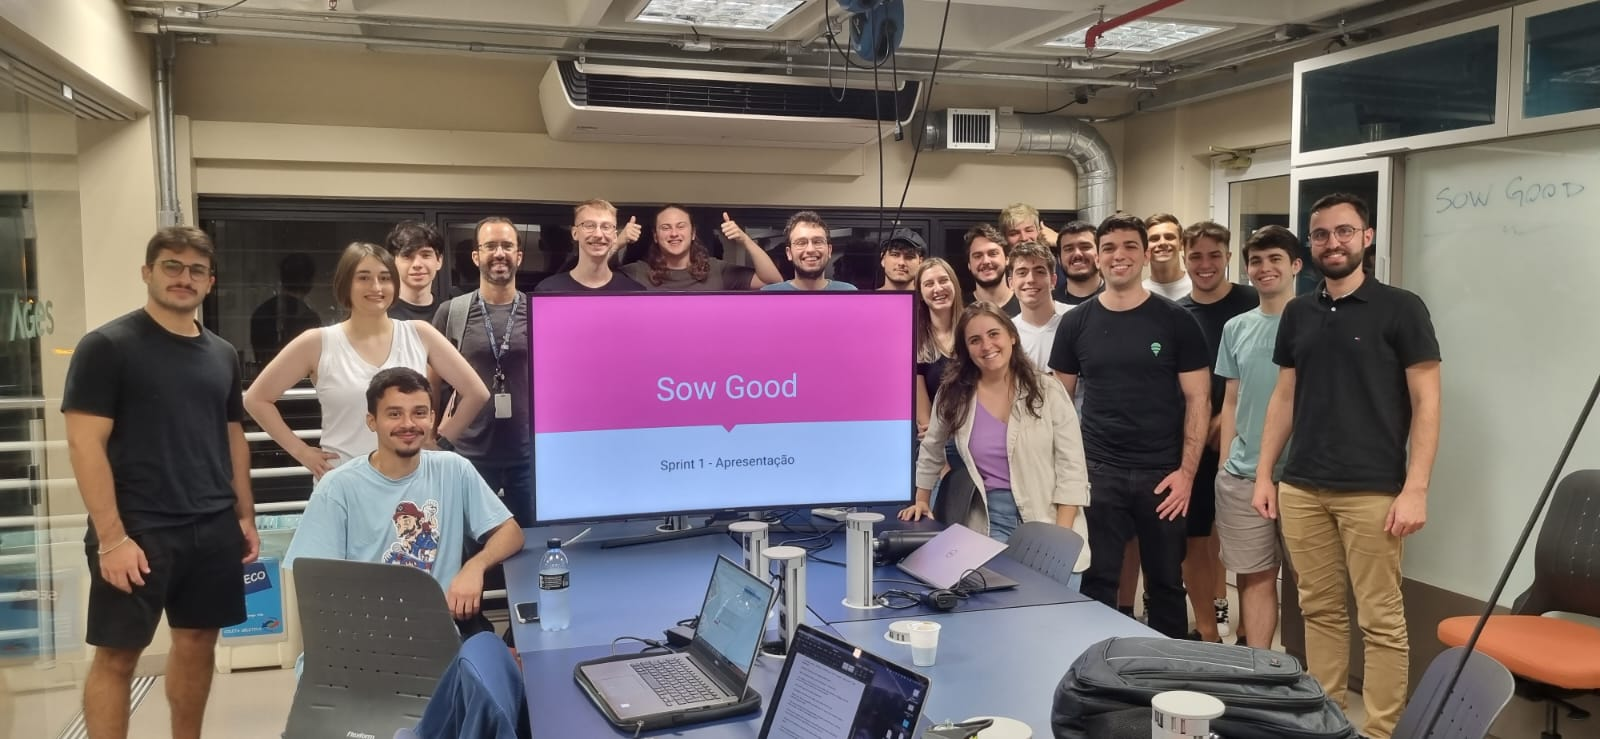
\includegraphics[width=1\linewidth]{conteudo//3 - ages II//conteudo//figures//foto-time.png}
    Fonte: https://tools.ages.pucrs.br/sow-good/wiki/-/wikis/home
\end{figure}